% ============================================================
% Artículo Científico - Serie Científica UCI
% Plantilla basada en: Omarmar, SC2025_V1
% Autor: Ruslan Alexei Martinez Campos
% ============================================================
\documentclass[12pt,a4paper]{article}

% --- Fuentes tipográficas ---
\usepackage{mathptmx}   % Times New Roman
\usepackage{helvet}     % Arial/Helvetica para títulos
\usepackage[T1]{fontenc}
\usepackage[utf8]{inputenc}
\usepackage[spanish,es-tabla]{babel}

% --- Espaciado y márgenes ---
\usepackage{setspace}
\onehalfspacing
\usepackage[top=3cm, bottom=3.5cm, left=2.5cm, right=2.5cm, headheight=48pt, footskip=2cm]{geometry}

% --- Gráficos y tablas ---
\usepackage{graphicx}
\usepackage{float}
\usepackage{longtable}
\usepackage{array}
\usepackage{multirow}
\usepackage{tabularx}
\usepackage{booktabs}

% --- Referencias ---
\usepackage[round,authoryear]{natbib}

% --- Otros ---
\usepackage{url}
\usepackage{xcolor}
\definecolor{darkblue}{RGB}{0,0,128}
\usepackage{hyperref}
\hypersetup{
    colorlinks=true,
    linkcolor=black,
    citecolor=black,
    urlcolor=blue
}

% --- Encabezado y pie de página (estilo revista) ---
\usepackage{fancyhdr}
\pagestyle{fancy}
\fancyhf{}
\renewcommand{\headrulewidth}{0.4pt}
\renewcommand{\headrule}{%
  \hrule width \headwidth height \headrulewidth \vskip -\baselineskip
}
\renewcommand{\footrulewidth}{0pt}
\lhead{\scriptsize\sffamily
  ISSN: 2306-2495 | RNPS: 2343\\
  http://publicaciones.uci.cu}
\rhead{\scriptsize\sffamily\raggedleft
  Serie Científica de la Universidad de las Ciencias Informáticas\\
  Vol.~19, No.~2, Mes: Abril-Junio, 2026, Pág.~1-15}
\fancyfoot[L]{\footnotesize
  \begin{minipage}[t]{0.9\textwidth}
    
\includegraphics[height=1.4em]{Images/cc.jpg}\hspace{0.3em}%
    Esta obra está bajo una licencia \textit{Creative Commons} de tipo Atribución 4.0 Internacional (CC BY 4.0)\\
    Grupo Editorial ``Ediciones Futuro'' Universidad de las Ciencias Informáticas. La Habana, Cuba \href{mailto:seriecientifica@uci.cu}{seriecientifica@uci.cu}
  \end{minipage}}
\fancyfoot[R]{\thepage}
% Redefinir estilo plain (páginas con \section*) para que también tenga encabezado
\fancypagestyle{plain}{%
  \fancyhf{}
  \renewcommand{\headrulewidth}{0.4pt}
  \renewcommand{\headrule}{%
    \hrule width \headwidth height \headrulewidth \vskip -\baselineskip
  }
  \lhead{\scriptsize\sffamily
    ISSN: 2306-2495 | RNPS: 2343\\
    http://publicaciones.uci.cu}
  \rhead{\scriptsize\sffamily\raggedleft
    Serie Científica de la Universidad de las Ciencias Informáticas\\
    Vol.~19, No.~2, Mes: Abril-Junio, 2026, Pág.~1-15}
  \fancyfoot[L]{\footnotesize
    \begin{minipage}[t]{0.9\textwidth}
      
\includegraphics[height=1.4em]{Images/cc.jpg}\hspace{0.3em}%
      Esta obra está bajo una licencia \textit{Creative Commons} de tipo Atribución 4.0 Internacional (CC BY 4.0)\\
      Grupo Editorial ``Ediciones Futuro'' Universidad de las Ciencias Informáticas. La Habana, Cuba \href{mailto:seriecientifica@uci.cu}{seriecientifica@uci.cu}
    \end{minipage}}
  \fancyfoot[R]{\thepage}
}

% --- Formato de secciones (tamaños exactos según plantilla) ---
\usepackage{titlesec}
% Section: Arial Bold 16pt centrado, color azul oscuro
\titleformat{\section}
  {\rmfamily\bfseries\fontsize{16pt}{19pt}\selectfont\centering\color{darkblue}}
  {}{0em}{}[\vspace{-0.2em}]
\titlespacing*{\section}{0pt}{2.5ex}{1.5ex plus .2ex}

% Subsection: Arial Bold 14pt centrado, color azul oscuro
\titleformat{\subsection}
  {\rmfamily\bfseries\fontsize{14pt}{17pt}\selectfont\centering\color{darkblue}}
  {}{0em}{}[\vspace{-0.2em}]
\titlespacing*{\subsection}{0pt}{1.2ex}{1.2ex plus .2ex}

% Subsubsection: Arial Bold 13pt centrado, color azul oscuro
\titleformat{\subsubsection}
  {\rmfamily\bfseries\fontsize{13pt}{15.5pt}\selectfont\centering\color{darkblue}}
  {}{0em}{}[\vspace{-0.2em}]
\titlespacing*{\subsubsection}{0pt}{1.0ex}{1.0ex plus .2ex}

% --- Formato de figuras: Fig. X – Título ---
\usepackage{caption}
\DeclareCaptionLabelFormat{figlabel}{\textbf{\textsf{Fig.~#2}} --}
\DeclareCaptionLabelFormat{tablabel}{\textsf{\bothIfFirst{#1}{ }#2} --}
\captionsetup[figure]{labelformat=figlabel,labelsep=none,font=small,justification=centering}
\captionsetup[table]{labelformat=tablabel,labelsep=none,font=small,justification=centering,labelfont={sf},textfont={rm}}

% --- Formato de tabla (9pt contenido, 11pt título) ---
\usepackage{etoolbox}
\AtBeginEnvironment{longtable}{\small}
\AtBeginEnvironment{tabular}{\small}

% --- Sin numeración de secciones (artículo, no tesis) ---
\setcounter{secnumdepth}{0}

% ============================================================
\begin{document}

% --- TIPO DE ARTÍCULO ---
\begin{flushleft}
\textit{Tipo de artículo: Artículo original}
\end{flushleft}

\vspace{0.5cm}

% --- TÍTULO ORIGINAL (Arial Bold 14pt, centrado) ---
\begin{center}
{\sffamily\bfseries\Large Videojuego educativo para la promoción de los Objetivos de Desarrollo Sostenible mediante Aprendizaje Basado en Juegos}
\end{center}

\vspace{0.3cm}

% --- TRADUCCIÓN DEL TÍTULO (Arial sin negrita 14pt, centrado) ---
\begin{center}
{\sffamily\Large Educational Video Game for Promoting the Sustainable Development Goals through Game-Based Learning}
\end{center}

\vspace{0.5cm}

% --- AUTORES ---
\begin{flushleft}
Ruslan Alexei Martinez Campos\textsuperscript{1*}, \href{https://orcid.org/0009-0008-6831-4221}{https://orcid.org/0009-0008-6831-4221}\\
Juan Antonio Plasencia Soler\textsuperscript{2}, \href{https://orcid.org/0000-0002-0951-2403}{https://orcid.org/0000-0002-0951-2403}
\end{flushleft}

\vspace{0.3cm}

% --- AFILIACIONES ---
\begin{flushleft}
\textsuperscript{1} Facultad de Tecnologías Interactivas, Universidad de las Ciencias Informáticas, La Habana, Cuba.\\
\textsuperscript{2} Facultad de Informática Organizacional, Universidad de las Ciencias Informáticas, La Habana, Cuba.
\end{flushleft}

\vspace{0.1cm}

\begin{flushleft}
*Autor para la correspondencia: \textit{acampos@estudiantes.uci.cu}\textsuperscript{1}, \textit{juanps@uci.cu}\textsuperscript{2}
\end{flushleft}

\newpage

% ============================================================
% RESUMEN (Arial Bold Izq.)
% ============================================================
\noindent{\sffamily\bfseries RESUMEN}

\vspace{0.2cm}

El desconocimiento sobre los Objetivos de Desarrollo Sostenible de las Naciones Unidas dificulta que la población participe de forma activa en la Agenda 2030 y tome decisiones informadas en torno a la sostenibilidad. Los videojuegos educativos, sobre todo los basados en el Aprendizaje Basado en Juegos, han probado ser herramientas pedagógicas capaces de generar experiencias inmersivas que favorecen el aprendizaje significativo. Este trabajo tuvo como objetivo desarrollar un videojuego educativo a partir de la adaptación digital del juego de mesa oficial \textit{Go Goals!} de las Naciones Unidas, con el fin de promover el conocimiento de los 17 Objetivos de Desarrollo Sostenible. Se aplicó la metodología ágil Extreme Programming durante las fases de planificación, diseño e implementación, empleando el motor Godot Engine y el lenguaje GDScript para lograr una solución multiplataforma y con contenido educativo ampliable mediante archivos JSON. El resultado fue \textit{Go Goals! Digital}, un videojuego que incorpora mecánicas de tablero hexagonal, preguntas organizadas por Objetivos de Desarrollo Sostenible con retroalimentación inmediata y un módulo de estadísticas de aprendizaje. La validación incluyó pruebas unitarias, pruebas de aceptación y un cuestionario de satisfacción aplicado a diez usuarios, con un índice de satisfacción del cliente del 98,18\%. Estos resultados respaldan la viabilidad de digitalizar recursos educativos analógicos sobre sostenibilidad y muestran que la combinación del Aprendizaje Basado en Juegos con la Teoría del Flujo y el Modelo de Conocimiento Tecnológico, Pedagógico y del Contenido puede producir experiencias de aprendizaje efectivas.

\vspace{0.3cm}

\noindent{\sffamily\bfseries Palabras clave:} Aprendizaje Basado en Juegos; Objetivos de Desarrollo Sostenible; Godot Engine; videojuegos educativos; gamificación.

\newpage

% ============================================================
% ABSTRACT (Arial Bold Izq.)
% ============================================================
\noindent{\sffamily\bfseries ABSTRACT}

\vspace{0.2cm}

{\itshape
The widespread lack of knowledge about the United Nations' Sustainable Development Goals limits active engagement with the 2030 Agenda and hinders informed decision-making on sustainability. Educational video games, particularly those grounded in Game-Based Learning, constitute effective pedagogical tools that generate immersive experiences to facilitate meaningful learning. This study aimed to develop an educational video game based on the digital adaptation of the official United Nations board game \textit{Go Goals!}, designed to promote knowledge of the 17 Sustainable Development Goals. The Extreme Programming agile methodology was employed through its planning, design, and implementation phases, using Godot Engine and the GDScript language to produce a cross-platform, accessible solution with educational content extensible through JSON files. The result was the video game \textit{Go Goals! Digital}, which integrates hexagonal board mechanics, a Sustainable Development Goal-specific question system with immediate feedback, and a learning statistics module. Validation was carried out through unit tests, acceptance tests, and a satisfaction questionnaire administered to a sample of ten users, achieving a Customer Satisfaction Score of 98.18\%. These results confirm the viability and pedagogical relevance of digitizing analog educational resources on sustainability and demonstrate that the integration of theoretical frameworks such as Game-Based Learning, Flow Theory, and the Technological Pedagogical Content Knowledge Model produces effective and motivating learning experiences.\par}

\vspace{0.3cm}

\noindent{\sffamily\bfseries\itshape Keywords:} \textit{Game-Based Learning; Sustainable Development Goals; Godot Engine; educational video games; gamification.}

\vspace{0.5cm}

\hrule
\vspace{0.5cm}

\newpage

% ============================================================
% INTRODUCCIÓN (Arial Bold 16pt, centrado)
% ============================================================
\section{Introducción}

La sostenibilidad se entiende como la capacidad de satisfacer las necesidades presentes sin comprometer las de generaciones futuras. Involucra la interrelación entre desarrollo económico, inclusión social y protección ambiental \citep{WCED1987}. En ese marco, la Educación para el Desarrollo Sostenible (EDS) busca formar ciudadanos capaces de participar en la construcción de sociedades más justas, lo que conecta directamente con los Objetivos de Desarrollo Sostenible (ODS) adoptados por las Naciones Unidas en 2015 como parte de la Agenda 2030 \citep{NacionesUnidas2015, UNESCO2020EDS}.

Sin embargo, a pesar de la importancia de estos objetivos globales, las brechas educativas siguen siendo un problema serio. En 2021, unos 244 millones de niños y jóvenes se encontraban fuera del sistema escolar en el mundo \citep{GlobalEduReport2022}, y en América Latina la falta de dispositivos y conectividad afectó directamente la continuidad de la educación \citep{BancoMundial2025}. El caso de Cuba ilustra esta paradoja. Con un 99,7\% de alfabetización en la población adulta \citep{UNESCO2023} y educación gratuita en todos los niveles \citep{CubaConstitucion2019}, el país enfrenta, sin embargo, la escasez de materiales didácticos digitales y serias limitaciones de conectividad. Aunque existen iniciativas de informatización escolar \citep{InformeVoluntarioCuba2021}, el desarrollo de software interactivo enfocado en los ODS apenas comienza.

Como alternativa para enfrentar dichos desafíos, los videojuegos educativos ofrecen un camino prometedor. Llevar un juego de mesa al entorno digital permite conservar su valor pedagógico mientras se aprovechan las ventajas de la interactividad, la retroalimentación inmediata y la eliminación de barreras logísticas \citep{MartinezGimenes2023}. A nivel internacional, las propias Naciones Unidas crearon el juego de mesa \textit{Go Goals!} como herramienta oficial para acercar los 17 ODS a niños de entre ocho y diez años, con una mecánica inspirada en el clásico Serpientes y Escaleras \citep{GoGoals2020}.

El Aprendizaje Basado en Juegos (ABJ) ha mostrado resultados positivos en entornos educativos formales, con mejoras apreciables en el rendimiento académico y en la transferencia de conocimientos a situaciones prácticas \citep{AguileraRoock2022}. El ABJ aprovecha recursos como la narrativa inmersiva, la retroalimentación adaptativa y la colaboración en tiempo real para aumentar la participación y la retención de conceptos \citep{Mabalay2025}. Algunos estudios recientes muestran que videojuegos como \textit{Eco} o \textit{Fate of the World} logran convertir información abstracta sobre sostenibilidad en experiencias concretas \citep{FernandezGaleote2021, FloodCradock2024}, y que títulos como \textit{Cities: Skylines} permiten al jugador experimentar cómo sus acciones individuales generan impactos a nivel sistémico \citep{Hawlitschek2022}.

La versión física de \textit{Go Goals!} presenta, sin embargo, limitaciones difíciles de ignorar: apenas 34 preguntas fijas que reducen la rejugabilidad, dependencia de la impresión a color, ninguna posibilidad de evaluar el aprendizaje y ausencia de mecanismos para jugar a distancia. Todo esto restringe su impacto pedagógico y complica su uso en contextos con pocos recursos. Hasta donde se ha podido constatar, no existe en Cuba ningún videojuego dedicado exclusivamente a enseñar los ODS mediante mecánicas de tablero digital.

De ahí la pregunta de investigación: ¿cómo contribuir a la enseñanza de los Objetivos de Desarrollo Sostenible? El objetivo general fue desarrollar un videojuego educativo basado en la adaptación digital de \textit{Go Goals!} que contribuyera a promover los ODS, usando la metodología Extreme Programming y el motor Godot Engine para lograr una solución accesible, multiplataforma y con contenido educativo ampliable.

\vspace{0.3cm}

A continuación se presenta la metodología de la investigación, que abarca los marcos teóricos, el análisis del referente analógico, la metodología de desarrollo y las tecnologías empleadas; luego se exponen los principales resultados obtenidos y su discusión; y finalmente se presentan las conclusiones del trabajo.

% ============================================================
% METODOLOGÍA
% ============================================================
\section{Metodología}

\subsection{Marco pedagógico del Aprendizaje Basado en Juegos}

El diseño del videojuego se apoyó en tres marcos teóricos que cubren los aspectos pedagógicos, tecnológicos y disciplinares del proyecto. El Aprendizaje Basado en Juegos (ABJ), o \textit{Game-Based Learning} en inglés, es la metodología central y consiste en utilizar sistemas interactivos completos como eje del proceso formativo \citep{PlassHomer2020}. A diferencia de la gamificación, que se limita a añadir mecánicas de recompensa en contextos no lúdicos \citep{Mabalay2025}, el ABJ construye una simulación integral donde el aprendizaje forma parte orgánica de la dinámica del juego \citep{AguileraRoock2022}.

La Teoría del Flujo \citep{Csikszentmihalyi1990} guió decisiones sobre el ritmo, la dificultad progresiva y la retroalimentación del juego. Según Csikszentmihalyi, los entornos lúdicos mantienen la motivación cuando hay equilibrio entre el desafío y la habilidad del jugador, lo que genera un estado de inmersión favorable para aprender. El Modelo TPACK \citep{MishraKoehler2006} sirvió para articular los tres dominios del proyecto: el conocimiento sobre los ODS, es decir, el contenido disciplinar; las orientaciones metodológicas de enseñanza, o conocimiento pedagógico; y las capacidades técnicas de Godot, o conocimiento tecnológico.

% *** RECOMENDACIÓN DE IMAGEN 1 ***
% Se recomienda incluir aquí un diagrama conceptual que muestre la
% intersección de los tres marcos teóricos: ABJ, Teoría del Flujo y
% Modelo TPACK, aplicados al diseño del videojuego.
% Esta imagen existe en la tesis: Images/Relación ABJ, TPACK y Gamificación.jpg
% Descomente las líneas siguientes para incluirla:
%
% \begin{figure}[H]
%   \centering
%   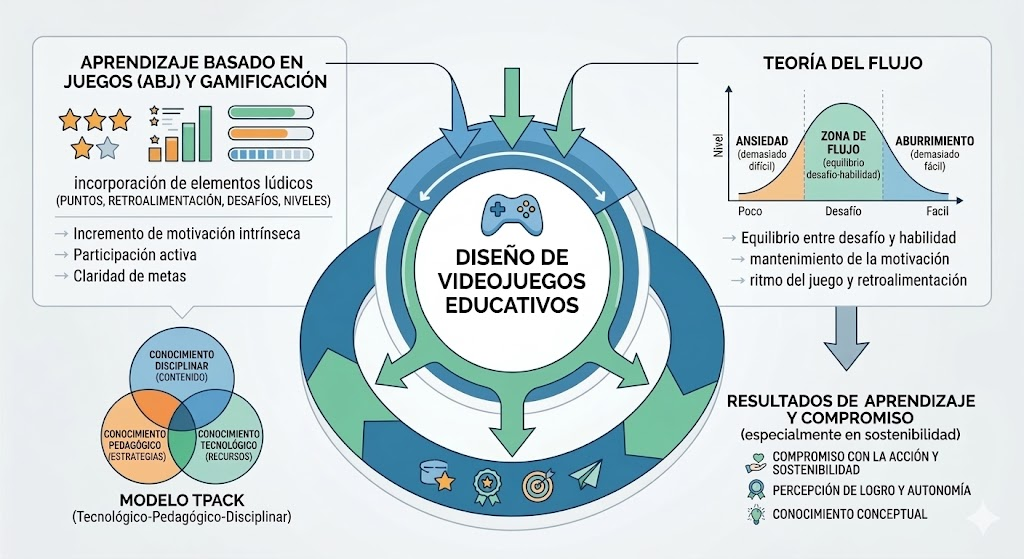
\includegraphics[width=0.65\textwidth]{Images/Relación ABJ, TPACK y Gamificación.jpg}
%   \caption{Intersección de los marcos teóricos ABJ, TPACK y Gamificación aplicados al diseño del videojuego educativo (elaboración propia).}
%   \label{fig:marcos_teoricos}
% \end{figure}

\subsection{Análisis del referente analógico y soluciones homólogas}

El juego de mesa \textit{Go Goals!} es un recurso educativo oficial de las Naciones Unidas dirigido a poblaciones infantiles \citep{GoGoals2020}. Tiene un tablero de 63 casillas hexagonales que representan el camino hacia el año 2030, con 17 casillas temáticas, una por cada ODS, donde los jugadores responden preguntas de opción múltiple. Dichas preguntas siguen la taxonomía de Bloom, pasando de la comprensión básica al análisis y la aplicación.

Del análisis del referente analógico salieron fortalezas claras: mecánicas pedagógicas probadas, lenguaje accesible y una progresión cognitiva bien estructurada. Pero también limitaciones que justifican la adaptación digital: solo 34 preguntas fijas que reducen la rejugabilidad, dependencia de la impresión a color, imposibilidad de usarlo en educación a distancia y falta de registro del aprendizaje individual.

Para contextualizar la propuesta y verificar su originalidad se analizaron cinco videojuegos que guardan relación con el proyecto. \textit{World Rescue}, oficial de Naciones Unidas, se basa en minijuegos de resolución de problemas; \textit{Trivia Crack} aporta la referencia mecánica de preguntas y respuestas; la serie \textit{Mario Party} sirve como referencia lúdica de tablero digital; \textit{Alba: A Wildlife Adventure} es una aventura centrada en los ODS 14 y 15; y \textit{Bleentoro} plantea un rompecabezas enfocado en los ODS 9 y 12. La comparación arrojó una brecha clara: las soluciones comerciales tienen buenas mecánicas lúdicas pero carecen de contenido educativo sobre sostenibilidad, mientras que los juegos enfocados en ODS recurren a minijuegos desconectados sin la cohesión metafórica del tablero original. Esta brecha justificó la necesidad de crear un recurso que llevara la mecánica de \textit{Go Goals!} a una plataforma digital completa.

\subsection{Metodología de desarrollo de software}

Para gestionar el ciclo de vida del producto se adoptó Extreme Programming (XP), una metodología ágil iterativa que se remonta a la década de 1990 \citep{Beck2004} y que promueve iteraciones cortas, fuerte orientación al cliente, simplicidad en la arquitectura y escalamiento constante del prototipo. Sus valores fundamentales son la comunicación, la simplicidad, la retroalimentación y el coraje. Estos encajaron bien con las condiciones de un desarrollo unipersonal sobre un motor gráfico, donde la validación visual continua y las refactorizaciones inmediatas son parte del día a día \citep{Sommerville2021}.

El desarrollo se dividió en cinco iteraciones con una progresión lógica. Las dos primeras cubrieron lo esencial: menú principal, instrucciones, inicio de partida, visualización del tablero, dado y movimiento de fichas. La tercera integró el núcleo pedagógico: sistema de preguntas ODS, evaluación de respuestas y gestión de turnos. La cuarta añadió funcionalidades de cierre como victoria, estadísticas, audio y pausa. La quinta incorporó características complementarias: cámara de seguimiento y modo de práctica. Al terminar cada iteración se ejecutaron pruebas de aceptación para validar los criterios establecidos.

\subsection{Selección de tecnologías y herramientas}

La selección del motor se basó en una comparativa técnica según criterios de licenciamiento, soporte 2D, exportación multiplataforma y curva de aprendizaje. Se optó por Godot Engine v4.6.2 \citep{GodotEngine2026} por su licencia MIT, su arquitectura modular basada en nodos y escenas, su motor 2D eficiente, la exportación nativa a Windows, Linux y macOS, y el uso de GDScript, lenguaje similar a Python que agiliza el prototipado \citep{Vanhove2024, GodotDocs2026}. Se descartaron Unity, por la inestabilidad de sus políticas de licenciamiento y su sobrecarga para proyectos 2D; Unreal Engine, orientado a gráficos 3D fotorrealistas con altos requerimientos de hardware; y Construct 3, de modelo por suscripción y enfocado en entornos web.

El resto del ecosistema de herramientas incluyó Visual Paradigm para el modelado UML \citep{Pressman2019}, Inkscape para los activos gráficos vectoriales, Git para el control de versiones \citep{Sommerville2021} y GitHub Projects para la gestión ágil mediante tableros Kanban.

% ============================================================
% RESULTADOS Y DISCUSIÓN
% ============================================================
\section{Resultados y discusión}

\subsection{Descripción de la solución: Go Goals! Digital}

\textit{Go Goals! Digital} es un videojuego educativo basado en la adaptación digital del juego de mesa oficial \textit{Go Goals!} de las Naciones Unidas. En su formato digital, de uno a cuatro jugadores controlan fichas sobre un tablero hexagonal de 63 casillas que metaforiza el recorrido colectivo hacia el año 2030, horizonte establecido por la Agenda 2030 para el Desarrollo Sostenible. El avance se determina mediante un dado virtual de seis caras, y al caer en una de las 17 casillas temáticas, una por cada ODS, el jugador debe responder una pregunta de opción múltiple sobre el objetivo correspondiente. Las respuestas correctas activan el efecto de escalera, que produce un avance positivo, mientras que las incorrectas activan el efecto de serpiente, que implica un retroceso correctivo. Así se preserva la mecánica pedagógica central del juego original.

\begin{figure}[H]
  \centering
  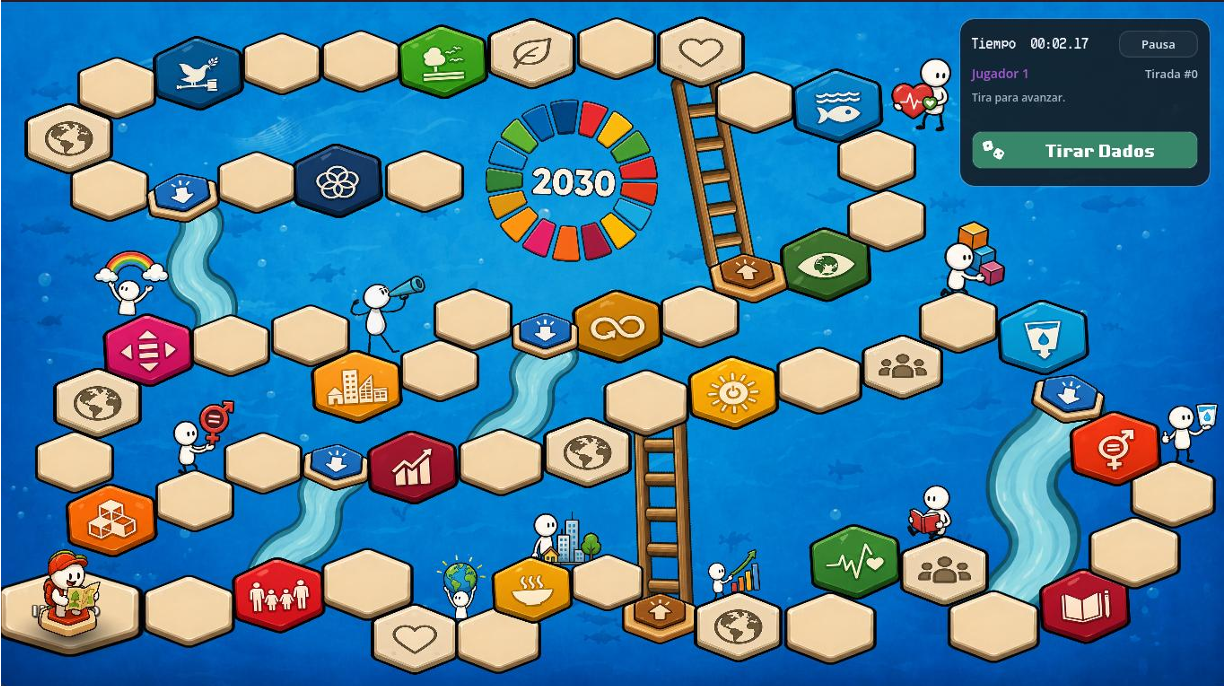
\includegraphics[width=0.80\textwidth]{Images/GoGoals Digital.png}
  \caption{Vista general del tablero de juego en \textit{Go Goals! Digital}, con el recorrido hexagonal de 63 casillas y las 17 casillas temáticas de los ODS (elaboración propia).}
  \label{fig:tablero_digital}
\end{figure}

La versión digital introduce varias mejoras frente al formato físico: accesibilidad multiplataforma sin necesidad de materiales físicos, banco de preguntas ampliable en JSON editable por educadores sin saber programar, retroalimentación visual y sonora inmediata, registro automático de aciertos y errores por jugador y por ODS, y selección aleatoria sin repetición de preguntas durante cada sesión para favorecer la rejugabilidad.

% *** RECOMENDACIÓN DE IMAGEN 2 ***
% Se recomienda incluir aquí un diagrama de arquitectura del sistema que
% muestre la jerarquía de nodos de Godot y los componentes principales:
% GameManager, GameEvents, GameState, GameData, AudioManager.
% Esta imagen existe en la tesis: Images/SceeneTree.jpg
% Descomente las líneas siguientes para incluirla:
%
% \begin{figure}[H]
%   \centering
%   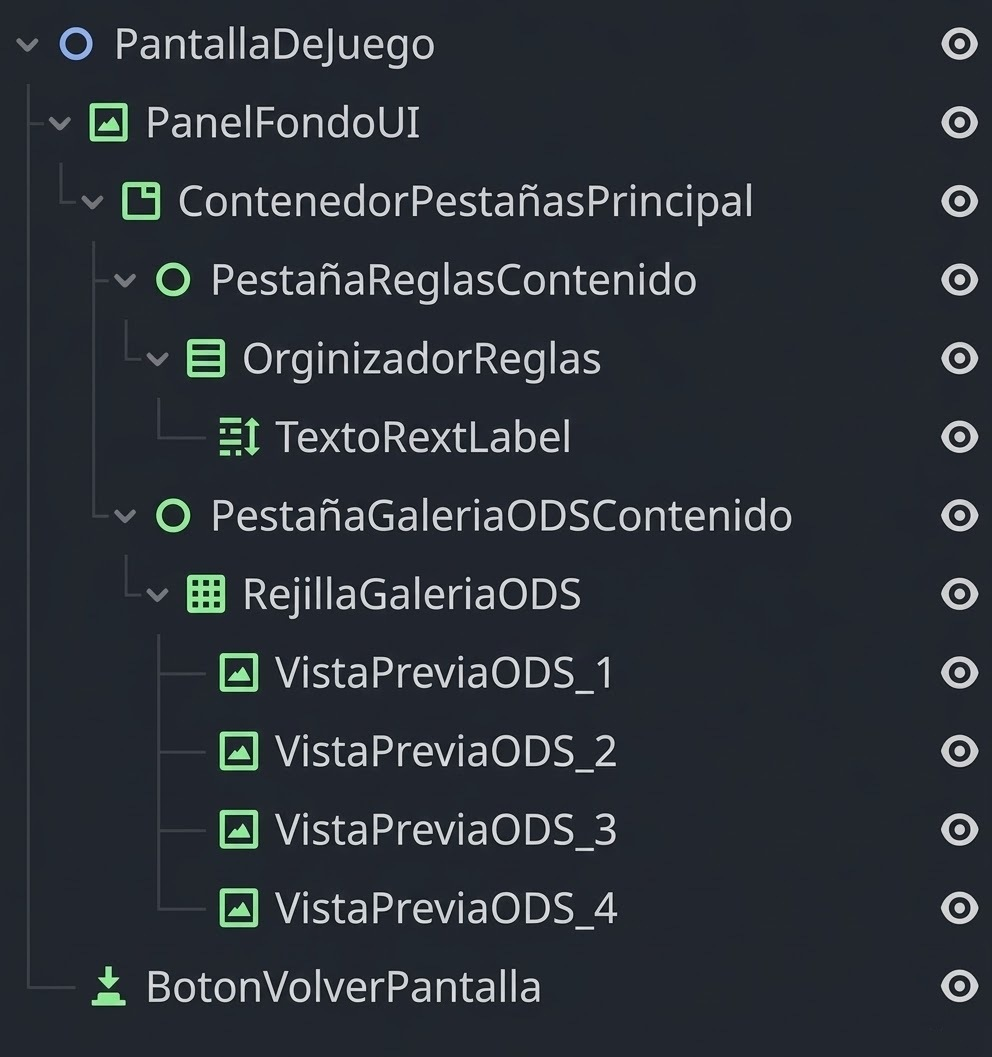
\includegraphics[width=0.55\textwidth]{Images/SceeneTree.jpg}
%   \caption{Jerarquía de nodos en el SceneTree de Godot: estructura arquitectónica del videojuego (elaboración propia).}
%   \label{fig:arquitectura}
% \end{figure}

\subsection{Diseño de la mecánica pedagógica}

El panel de preguntas es el componente central de la experiencia educativa. Aparece como interfaz modal que se superpone al tablero cuando el jugador cae en una casilla temática, pausando el juego para concentrar la atención en el contenido pedagógico. Al seleccionar una respuesta, el panel muestra un indicador visual claro: verde para respuestas correctas y rojo para incorrectas, junto con una breve explicación que refuerza lo aprendido, y permanece visible unos cinco segundos antes de cerrar y dar continuidad al turno.

\begin{figure}[H]
  \centering
  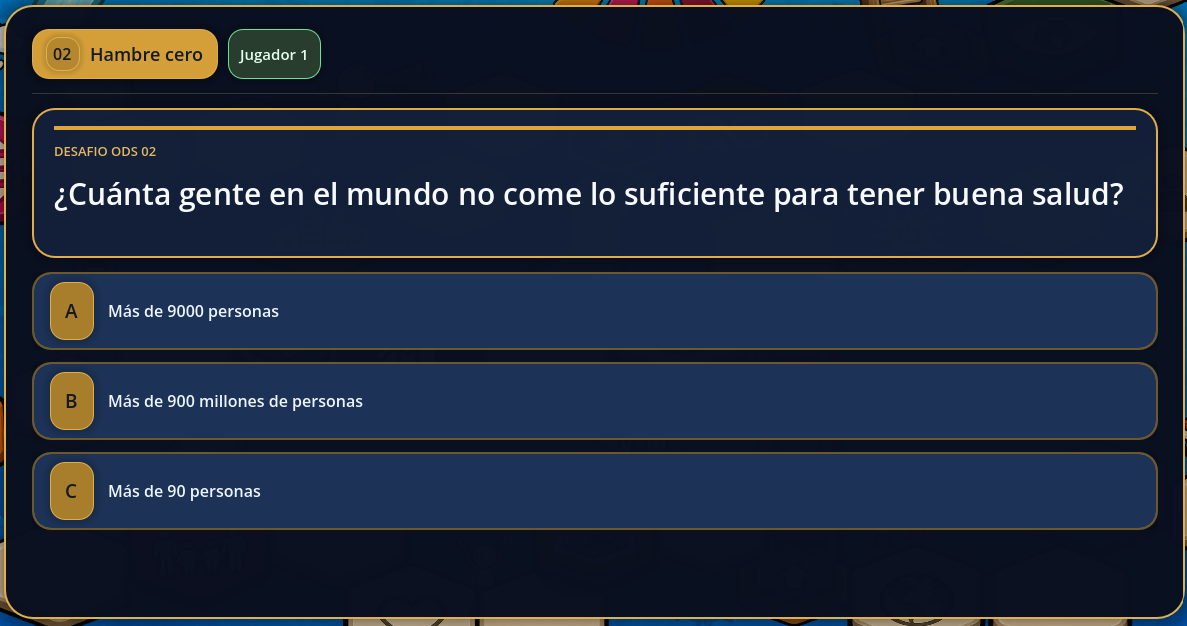
\includegraphics[width=0.70\textwidth]{Images/Panel Preguntas.png}
  \caption{Panel de preguntas educativas por ODS: interfaz modal con el ícono del objetivo, el enunciado de la pregunta y las opciones de respuesta de selección múltiple (elaboración propia).}
  \label{fig:panel_preguntas}
\end{figure}

La arquitectura del sistema se construyó sobre cuatro pilares: escenas independientes para cada funcionalidad, como menú, tablero y panel de preguntas; servicios globales mediante autocargas (\textit{autoloads}), como \texttt{GameData} para configuración y banco de preguntas, \texttt{AudioManager} para sonido y \texttt{RecordsManager} para persistencia; un controlador central \texttt{GameManager} que orquesta el ciclo de la partida; y un bus de señales globales en \texttt{GameEvents} que permite a los componentes comunicarse sin acoplamiento directo \citep{GodotDocs2026}.

El banco de preguntas se almacena en archivos JSON, lo que permite a educadores sin conocimientos de programación añadir, modificar o traducir preguntas con cualquier editor de texto. Esta decisión de diseño facilita la extensibilidad y la adaptación del recurso a diferentes contextos culturales y lingüísticos.

\subsection{Definición de requisitos}

Los requisitos se definieron mediante sesiones de trabajo con el cliente y el análisis de las mecánicas del juego original. Los 18 requisitos funcionales cubren desde la navegación básica (menú, instrucciones, inicio de partida) hasta las mecánicas del tablero hexagonal, el lanzamiento del dado, el movimiento animado de fichas y los efectos de escalera y serpiente. También abarcan el núcleo pedagógico —preguntas ODS con selección aleatoria, retroalimentación inmediata— y el cierre de la experiencia con gestión de turnos, detección de victoria, estadísticas y modo de práctica.

Los 13 requisitos no funcionales se dividieron en cuatro categorías que definieron los atributos de calidad del sistema: usabilidad con interfaz intuitiva, tipografía legible y contraste alto con los colores oficiales de los ODS; rendimiento con respuesta menor a 0,5 segundos y ejecutable bajo 150~MB; compatibilidad con Windows 10+, Linux Ubuntu 20.04+ y macOS 11+ en funcionamiento sin conexión; y hardware con procesador de doble núcleo a 1,5~GHz, 512~MB de RAM y 300~MB de almacenamiento.

\subsection{Validación del sistema}

La validación se hizo en tres niveles de pruebas, siguiendo las buenas prácticas de XP \citep{Pressman2019}. Las \textbf{pruebas unitarias} evaluaron de forma automatizada las funcionalidades críticas mediante el entorno Godot Unit Testing (GUT). Se diseñaron ocho casos de prueba para la recuperación de preguntas por ODS, verificando que el sistema devolviera preguntas del objetivo correcto, evitara repeticiones mientras hubiera preguntas disponibles y reiniciara el ciclo al agotarse el conjunto. Todos los casos pasaron con éxito.

Las \textbf{pruebas de aceptación} se ejecutaron al cierre de cada iteración, con 18 casos de prueba vinculados a las historias de usuario. Las iteraciones 1, 2, 4 y 5 obtuvieron 100\% de aprobación. En la iteración 3 se detectó un defecto en la historia de usuario 9, correspondiente a mostrar pregunta ODS: al superar los 50 caracteres, el texto de las opciones de respuesta se superponía con los bordes del panel. Se corrigió ajustando el tamaño de fuente y añadiendo saltos de línea automáticos, tras lo cual la iteración también alcanzó el 100\%.

\renewcommand{\arraystretch}{1.3}
\begin{longtable}{|c|c|c|c|}
\caption{Resumen de resultados de las pruebas de aceptación por iteración (elaboración propia).}
\label{tab:resultados_aceptacion}\\
\hline
\textbf{Iteración} & \textbf{Casos de prueba} & \textbf{Aprobación} & \textbf{No conformidades} \\
\hline
\endfirsthead
\multicolumn{4}{c}{\tablename\ \thetable{} -- Continuación}\\
\hline
\textbf{Iteración} & \textbf{Casos de prueba} & \textbf{Aprobación} & \textbf{No conformidades} \\
\hline
\endhead
\hline
\multicolumn{4}{r}{\small Continúa en la siguiente página...}\\
\endfoot
\hline
\endlastfoot
1 & 4 & 100\% & 0 \\
\hline
2 & 4 & 100\% & 0 \\
\hline
3 & 3 & 100\% & 0 \\
\hline
4 & 5 & 100\% & 0 \\
\hline
5 & 2 & 100\% & 0 \\
\hline
\textbf{Total} & \textbf{18} & \textbf{100\%} & \textbf{0} \\
\hline
\end{longtable}

% *** RECOMENDACIÓN DE IMAGEN 3 ***
% Se recomienda incluir aquí una captura de pantalla de los resultados
% de las pruebas unitarias en el framework GUT, que muestra los 8 casos
% de prueba exitosos (checks verdes).
% Esta imagen existe en la tesis: Images/Resultado de Prueba.png
% Descomente las líneas siguientes para incluirla:
%
% \begin{figure}[H]
%   \centering
%   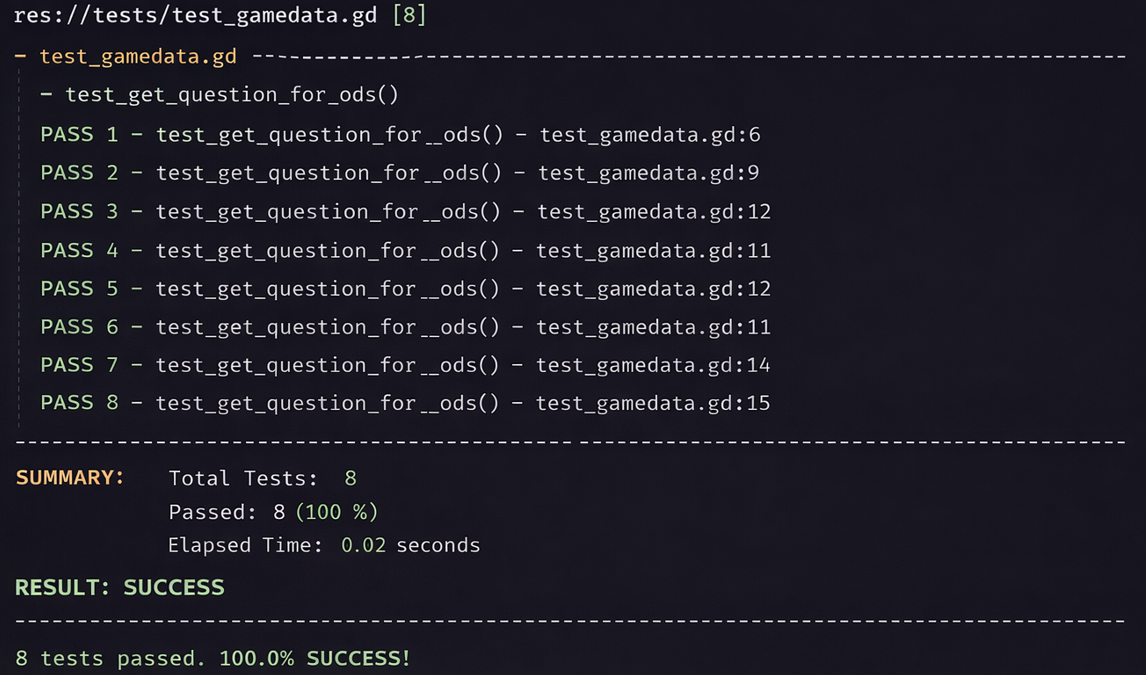
\includegraphics[width=0.60\textwidth]{Images/Resultado de Prueba.png}
%   \caption{Resultados de las pruebas unitarias automatizadas para la clase \texttt{GameData} utilizando el framework GUT (elaboración propia).}
%   \label{fig:pruebas_unitarias}
% \end{figure}

\subsection{Índice de aceptación del usuario}

Para medir la aceptación del usuario se trabajó con una muestra de diez estudiantes de La Habana, entre 15 y 25 años, a quienes se les distribuyó el videojuego. Se aplicó un cuestionario basado en escala de Likert (1--5) que evaluó cinco aspectos: experiencia general y jugabilidad, interfaz y diseño visual, rendimiento técnico, contenido educativo y relación con los ODS, y satisfacción global.

\renewcommand{\arraystretch}{1.3}
\begin{longtable}{|p{0.45\textwidth}|c|c|c|}
\caption{Resultados del cuestionario de satisfacción del usuario -- Go Goals! Digital (elaboración propia).}
\label{tab:resultados_csat}\\
\hline
\textbf{Categoría} & \textbf{Positivas} & \textbf{Neutrales} & \textbf{Negativas} \\
\hline
\endfirsthead
\multicolumn{4}{c}{\tablename\ \thetable{} -- Continuación}\\
\hline
\textbf{Categoría} & \textbf{Positivas} & \textbf{Neutrales} & \textbf{Negativas} \\
\hline
\endhead
\hline
\multicolumn{4}{r}{\small Continúa en la siguiente página...}\\
\endfoot
\hline
\endlastfoot
Experiencia General y Jugabilidad & 30 & 0 & 0 \\
\hline
Interfaz y Diseño Visual & 28 & 2 & 0 \\
\hline
Rendimiento Técnico & 10 & 0 & 0 \\
\hline
Contenido Educativo y ODS & 30 & 0 & 0 \\
\hline
Satisfacción Global & 10 & 0 & 0 \\
\hline
\textbf{Total} & \textbf{108} & \textbf{2} & \textbf{0} \\
\hline
\end{longtable}

El \textit{Customer Satisfaction Score} (CSAT), calculado como el porcentaje de respuestas positivas sobre el total, dio 108 positivas de 110 totales: un 98,18\%. Es un valor muy alto que respalda la calidad técnica, el diseño instruccional y la aceptación del videojuego por su público objetivo. Todos los evaluadores indicaron que lo recomendarían a otras personas interesadas en aprender sobre sostenibilidad.

\subsection{Discusión}

\textit{Go Goals! Digital} aporta una propuesta distinta dentro de los videojuegos educativos sobre ODS. Mientras que \textit{World Rescue}, por ejemplo, aborda los ODS con minijuegos desconectados entre sí, aquí el aprendizaje se integra en una mecánica de tablero cohesiva que metaforiza el camino hacia la Agenda 2030, manteniendo la fidelidad pedagógica del juego original de Naciones Unidas.

El 98,18\% de aceptación en el cuestionario CSAT está por encima de los valores que suele reportar la literatura para videojuegos educativos \citep{Hawlitschek2022}, lo que sugiere que combinar ABJ, Teoría del Flujo y Modelo TPACK dio buenos resultados. El hecho de que no hubiera respuestas negativas en cuatro de las cinco categorías indica que el diseño centrado en accesibilidad y retroalimentación inmediata funcionó bien para el público al que va dirigido.

Haber elegido Godot Engine, con su licencia MIT libre y capacidad de exportar a varias plataformas, resuelve varios problemas de accesibilidad del formato físico: ya no depende de la impresión a color, se puede distribuir gratis y funciona sin conexión a internet, algo especialmente útil en contextos educativos con conectividad limitada \citep{UNICEF2022}.

El banco de preguntas en JSON aborda directamente el problema del contenido estático del juego original, pues permite que educadores amplíen y adapten el contenido sin saber programar. Esto hace del videojuego un recurso que puede mejorarse de forma continua y adaptarse a distintos contextos culturales.

Comparado con enfoques puramente gamificados, donde se añaden mecánicas de juego en contextos que no lo son \citep{Mabalay2025}, el ABJ hace que el contenido educativo sea parte orgánica de la dinámica del juego: aprender no es una actividad aparte, sino el mecanismo central para avanzar. Esta integración, que encuentra respaldo en la Teoría del Flujo \citep{Csikszentmihalyi1990}, ayuda a explicar los altos niveles de satisfacción en experiencia general y contenido educativo.

% ============================================================
% CONCLUSIONES
% ============================================================
\section{Conclusiones}

El desarrollo de \textit{Go Goals! Digital} cumplió con el objetivo de contribuir a la promoción de los Objetivos de Desarrollo Sostenible mediante la adaptación digital del juego de mesa oficial de las Naciones Unidas. A continuación se presentan las conclusiones derivadas del trabajo:

El marco teórico construido sobre el ABJ, la Teoría del Flujo y el Modelo TPACK respaldó la pertinencia pedagógica de usar videojuegos para enseñar sostenibilidad, y sirvió de base científica para las decisiones de diseño.

El análisis de soluciones homólogas confirmó la originalidad de la propuesta: no se encontró ningún videojuego que adapte fielmente la mecánica de un juego de mesa oficial sobre ODS a un entorno digital interactivo. El diagnóstico del \textit{Go Goals!} físico puso en evidencia las limitaciones de accesibilidad, escalabilidad y rejugabilidad que justificaron su digitalización.

La metodología Extreme Programming, junto con Godot Engine y GDScript, permitió un desarrollo ágil con validación temprana de funcionalidades y ajustes continuos, lo que dio como resultado un producto con 100\% de aprobación en las pruebas de aceptación tras corregir el único defecto encontrado.

El 98,18\% de aceptación documentado con el cuestionario CSAT confirma que la solución cumple con lo que espera el público objetivo, y valida la combinación entre mecánicas lúdicas de tablero y contenido educativo sobre sostenibilidad.

Como trabajo futuro se prevé ampliar el banco de preguntas con distintos niveles de complejidad para diferentes edades; implementar un sistema de logros y recompensas virtuales; diseñar una arquitectura de red para modo multijugador en línea; y adaptar la interfaz a plataformas móviles, para ampliar el alcance del recurso educativo.

% ============================================================
% REFERENCIAS (Arial Bold 16pt, centrado)
% ============================================================
\bibliographystyle{apalike}
\bibliography{article_bib}

% ============================================================
% CONFLICTO DE INTERÉS
% ============================================================
\section*{Conflicto de interés}

El autor declara que no existen conflictos de interés que puedan haber influido en los resultados o la interpretación de este trabajo. El autor autoriza la distribución y uso de su artículo.

% ============================================================
% CONTRIBUCIONES DE LOS AUTORES
% ============================================================
\section*{Contribuciones de los autores}

\begin{enumerate}
    \item Conceptualización: Ruslan Alexei Martinez Campos.
    \item Curación de datos: Ruslan Alexei Martinez Campos.
    \item Análisis formal: Ruslan Alexei Martinez Campos.
    \item Investigación: Ruslan Alexei Martinez Campos.
    \item Metodología: Ruslan Alexei Martinez Campos.
    \item Administración del proyecto: Ruslan Alexei Martinez Campos.
    \item Software: Ruslan Alexei Martinez Campos.
    \item Supervisión: Juan Antonio Plasencia Soler, Oscar de Jesús Pacheco del Pino.
    \item Validación: Ruslan Alexei Martinez Campos.
    \item Visualización: Ruslan Alexei Martinez Campos.
    \item Redacción -- borrador original: Ruslan Alexei Martinez Campos.
    \item Redacción -- revisión y edición: Ruslan Alexei Martinez Campos.
\end{enumerate}

% ============================================================
% FINANCIACIÓN
% ============================================================
\section*{Financiación}

La investigación es financiada por el Proyecto: PS211LH008-011 ``Ecosistema de ciencia, tecnología e innovación para contribuir al cumplimiento de los Objetivos de Desarrollo Sostenible desde las instituciones de educación superior'' del Programa Sectorial de Ciencia, Tecnología e Innovación: ``Gestión de Ciencia, Tecnología e Innovación para el Desarrollo Sostenible''.

\end{document}
